\documentclass[12pt,preprint]{aastex}

% has to be before amssymb it seems
\usepackage{color,hyperref}
\definecolor{linkcolor}{rgb}{0,0,0.5}
\hypersetup{colorlinks=true,linkcolor=linkcolor,citecolor=linkcolor,
            filecolor=linkcolor,urlcolor=linkcolor}

\usepackage{url}
\usepackage{algorithmic,algorithm}
\usepackage{multirow}

\usepackage{listings}
\definecolor{lbcolor}{rgb}{0.9,0.9,0.9}
\lstset{language=Python,
        basicstyle=\footnotesize\ttfamily,
        showspaces=false,
        showstringspaces=false,
        tabsize=2,
        breaklines=false,
        breakatwhitespace=true,
        identifierstyle=\ttfamily,
        keywordstyle=\bfseries\color[rgb]{0.133,0.545,0.133},
        commentstyle=\color[rgb]{0.133,0.545,0.133},
        stringstyle=\color[rgb]{0.627,0.126,0.941},
    }

\newcommand{\dd}{\ensuremath{\,\mathrm{d}}}

\begin{document}

\title{%
Fitting a plane with arbitrary observational uncertainties
}

\newcommand{\nyu}{2}
\author{%
    Daniel~Foreman-Mackey\altaffilmark{1,\nyu}
}
\altaffiltext{1}{To whom correspondence should be addressed:
                        \url{danfm@nyu.edu}}
\altaffiltext{\nyu}{Center for Cosmology and Particle Physics,
                        Department of Physics, New York University,
                        4 Washington Place, New York, NY, 10003, USA}

% \begin{abstract}
% \end{abstract}
%
% \keywords{%
% }

In this note, I'll describe a method for inferring a planar relationship
between three variables given a set of noisy (and possibly non-Gaussian)
observations of a set of systems.
For specificity, consider the problem of gyrochronology: there is postulated
to be a linear relationship between the (true) age $A_n$ of a star $n$ and its
 (true) effective temperature $T_n$ and rotational period $P_n$
\begin{eqnarray}\label{eq:plane}
\log A_n &=& m_0 + m_1\,\log T_n + m_2\,\log P_n \quad.
\end{eqnarray}
We would like to determine the best-fit value (or sample the posterior
probability) of the parameter vector $m=\{m_0,m_1,m_2\}$ conditioned on a set
of noisy observations $\hat{A}_n$, $\hat{T}_n$, and $\hat{P}_n$.

For this purpose, we need to compute the marginalized likelihood
\begin{eqnarray}
p(\{\hat{A}_n,\hat{T}_n,\hat{P}_n\}\,|\,m) &=&
    \prod_{n=1}^N
        \int p(\hat{A}_n,\hat{T}_n,\hat{P}_n,A_n,T_n,P_n\,|\,m)
            \dd A_n \dd T_n \dd P_n \quad.
\end{eqnarray}
This joint probability function is shown in figure~\ref{fig:gm} and this
factorization can be written as
\begin{eqnarray}
p(\hat{A}_n,\hat{T}_n,\hat{P}_n,A_n,T_n,P_n\,|\,m) &=&
p(T_n)\,p(P_n)\,p(A_n\,|\,T_n,P_n,m)\,
    p(\hat{A}_n\,|\,A_n)\,p(\hat{T}_n\,|\,T_n)\,p(\hat{P}_n\,|\,P_n)
\nonumber
\end{eqnarray}
where (by equation~\ref{eq:plane})
\begin{eqnarray}
p(A_n\,|\,T_n,P_n,m) &=&
\delta \left [ \log A_n - (m_0 + m_1\,\log T_n + m_2\,\log P_n) \right] \quad.
\end{eqnarray}

Now, let's say that we have $J_n$ posterior samples
\begin{eqnarray}
T_n^{(j)} &\sim& p(T_n\,|\,\hat{T}_n) \nonumber \\
P_n^{(j)} &\sim& p(P_n\,|\,\hat{P}_n)
\end{eqnarray}
and that we can evaluate $p(\hat{A}_n\,|\,A_n)$ up to a normalization constant.
If you don't have the posterior samples, generate them from the uncertainties
provided in the catalog and if you don't have functional form for the age
likelihood, make one up using a KDE or similar.
Now, we can evaluate the marginalized likelihood for a single star very
efficiently as follows
\begin{eqnarray}
p(\hat{A}_n,\hat{T}_n,\hat{P}_n\,|\,m) &=&
\int
    p(T_n)\,p(P_n)\,p(A_n\,|\,T_n,P_n,m)\,
    p(\hat{A}_n\,|\,A_n)\,p(\hat{T}_n\,|\,T_n)\,p(\hat{P}_n\,|\,P_n)
    \dd A_n \dd T_n \dd P_n \nonumber\\
&\propto& \int
    p(A_n\,|\,T_n,P_n,m)\,p(\hat{A}_n\,|\,A_n)\,
    p(T_n\,|\,\hat{T}_n)\,p(P_n\,|\,\hat{P}_n)
    \dd A_n \dd T_n \dd P_n \nonumber\\
&\approx& \frac{1}{J_n} \sum_{j=1}^{J_n}p(\hat{A}_n\,|\,A_n^{(j)})
\end{eqnarray}
where $A_n^{(j)}$ is computed from the posterior samples using
equation~\ref{eq:plane}.

Finally, the full marginalized log-likelihood is
\begin{eqnarray}
\log p(\{\hat{A}_n,\hat{T}_n,\hat{P}_n\}\,|\,m) &\approx&
    \log\mathcal{Z} + \sum_{n=1}^N
        \log \left[ \sum_{j=1}^{J_n}p(\hat{A}_n\,|\,A_n^{(j)}) \right ]
\end{eqnarray}
where $\mathcal{Z}$ is an irrelevant normalization constant.
You can then toss this into an optimizer and find the maximum likelihood plane
or assert a prior $p(m)$ and draw posterior samples.

\begin{figure}[htbp]
\begin{center}
    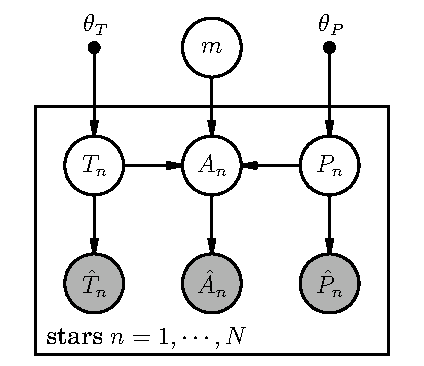
\includegraphics{pgm.pdf}
\end{center}
\caption{%
\label{fig:gm}}
\end{figure}

%\newcommand{\arxiv}[1]{\href{http://arxiv.org/abs/#1}{arXiv:#1}}
%\begin{thebibliography}{}\raggedright
%
%\bibitem[Fang \& Margot(2012)]{fang}
%Fang, J., \& Margot, J.-L.\ 2012, \apj, 761, 92
%\arxiv{1207.5250}
%
%\bibitem[Tremaine \& Dong(2012)]{tremaine}
%Tremaine, S., \& Dong, S.\ 2012, \aj, 143, 94
%\arxiv{1106.5403}
%
%\end{thebibliography}

\end{document}
